% ----------------------------------------------------------
\chapter{Metodologia
}\label{cap:desenvolvimento}
% ----------------------------------------------------------
\section{Interface gráfica}

A interface gráfica publicada no navegador foi elaborada utilizando CSS, JavaScript e HTML. 

\section{Representação tridimensional}

As representações tridimensionais moleculares foram feitas com Three.js, uma biblioteca que usa WebGL para desenhar (na realidade, renderizar) objetos 3D de maneira facilitada. No caso das moléculas, utilizamos modelos conhecidos, como o de bola (átomos) e bastões (ligações químicas) (do inglês \textit{ball and stick}), usado para exibir geometrias de moléculas em 3D. 

As esferas são comumente coloridas seguindo a convenção CPK (Corey-Pauling-Koltun), que se popularizou por distinguir bem os elementos químicos nos modelos moleculares. Em 1952, Corey e Pauling publicaram uma descrição dos modelos de preenchimento de espaço de proteínas e outras biomoléculas que eles haviam construído na Caltech \autocite{Corey1953}. Tal proposição foi melhorada em 1965, por Koltun, que estendeu essa técnica aos halogênios e metais \autocite{Crossland2004-ll}.

Várias das cores do CPK referem-se mnemonicamente às cores dos elementos puros ou compostos notáveis. Por exemplo, o hidrogênio é um gás incolor, o carbono como carvão vegetal, grafite ou coque é preto, o enxofre em pó é amarelo, o cloro é um gás esverdeado, o bromo é um líquido vermelho escuro, o iodo no éter é violeta, o fósforo amorfo é vermelho, a ferrugem é vermelho alaranjado escuro, etc. Para algumas cores, tais como as de oxigênio e nitrogênio, a inspiração é menos clara. Talvez o vermelho para oxigênio seja inspirado pelo fato de que o oxigênio é normalmente necessário para a combustão ou que o químico que contém oxigênio no sangue, hemoglobina, é vermelho vivo, e o azul para nitrogênio pelo fato de que o nitrogênio é o principal componente da atmosfera terrestre, que aos olhos humanos parece ser de cor azul céu.

É provável que as cores do CPK tenham sido inspiradas por modelos no século XIX. Em 1865, August Wilhelm von Hofmann, em uma palestra no \textit{Royal Institution} em Londres, estava usando modelos feitos de bolas de \textit{croquet} para ilustrar a valência, então ele usou as bolas coloridas disponíveis para ele. (Na época, o \textit{croquet} era o esporte mais popular na Inglaterra, portanto, as bolas eram abundantes). \textit{On the Combining Power of Atoms}, \textit{Chemical News}, 12 (1865, 176-9, 189, afirma que:

\begin{citacao}
Hofmann, em uma palestra dada na Royal Institution em abril de 1865 fez uso de bolas de croquete de diferentes cores para representar vários tipos de átomos (por exemplo, preto de carbono, branco de hidrogênio, verde de cloro, vermelho de oxigênio 'ardente', azul nitrogênio)\autocite{Crossland2004-ll}.
\end{citacao}

\section{Método de Hueckel Estendido}

O \gls{HMO} foi inicialmente proposto por Erich Hueckel em 1930 \autocite{Hckel1931} como uma alternativa para calcular orbitais moleculares como combinações lineares de orbitais atômicos\autocite{Coulson1978-ot}. Tal teoria prediz os orbitais moleculares de elétrons $\pi$ em moléculas com estrutura eletrônica deslocalizada., tal como o etileno, benzeno, butadieno e piridina. Isso nos fornece uma base teórica para fundamentar a regra de Hueckel, responsável por enunciar que moléculas cíclicas, planares ou espécies químicas iônicas com $4n + 2$ elétrons $\pi$ são aromáticos.

Esse modelo baseia-se no fato de que a interação entre dois orbitais atômicos (sobreposição) produz um orbital molecular ligante mais estável (energia mais baixa), e um orbital molecular antiligante, menos estável do que aqueles que o geraram. Dessa forma, o número de orbitais moleculares novos é igual ao número de orbitais atômicos envolvidos (a combinação linear). A estabilidade relativa ou as energias dos orbitais moleculares em um polieno completamente conjugado, cíclico, planar pode ser predita pela teoria de Hueckel. Tomando o benzeno como exemplo, é possível ilustrar, através de um círculo de Frost (\autoref{fig:M1}), os níveis de energia dos seus orbitais moleculares de fronteira.

\begin{figure}[htb]
	\caption{\label{fig:M1} Círculo de Frost para o benzeno.}
	\begin{center}
		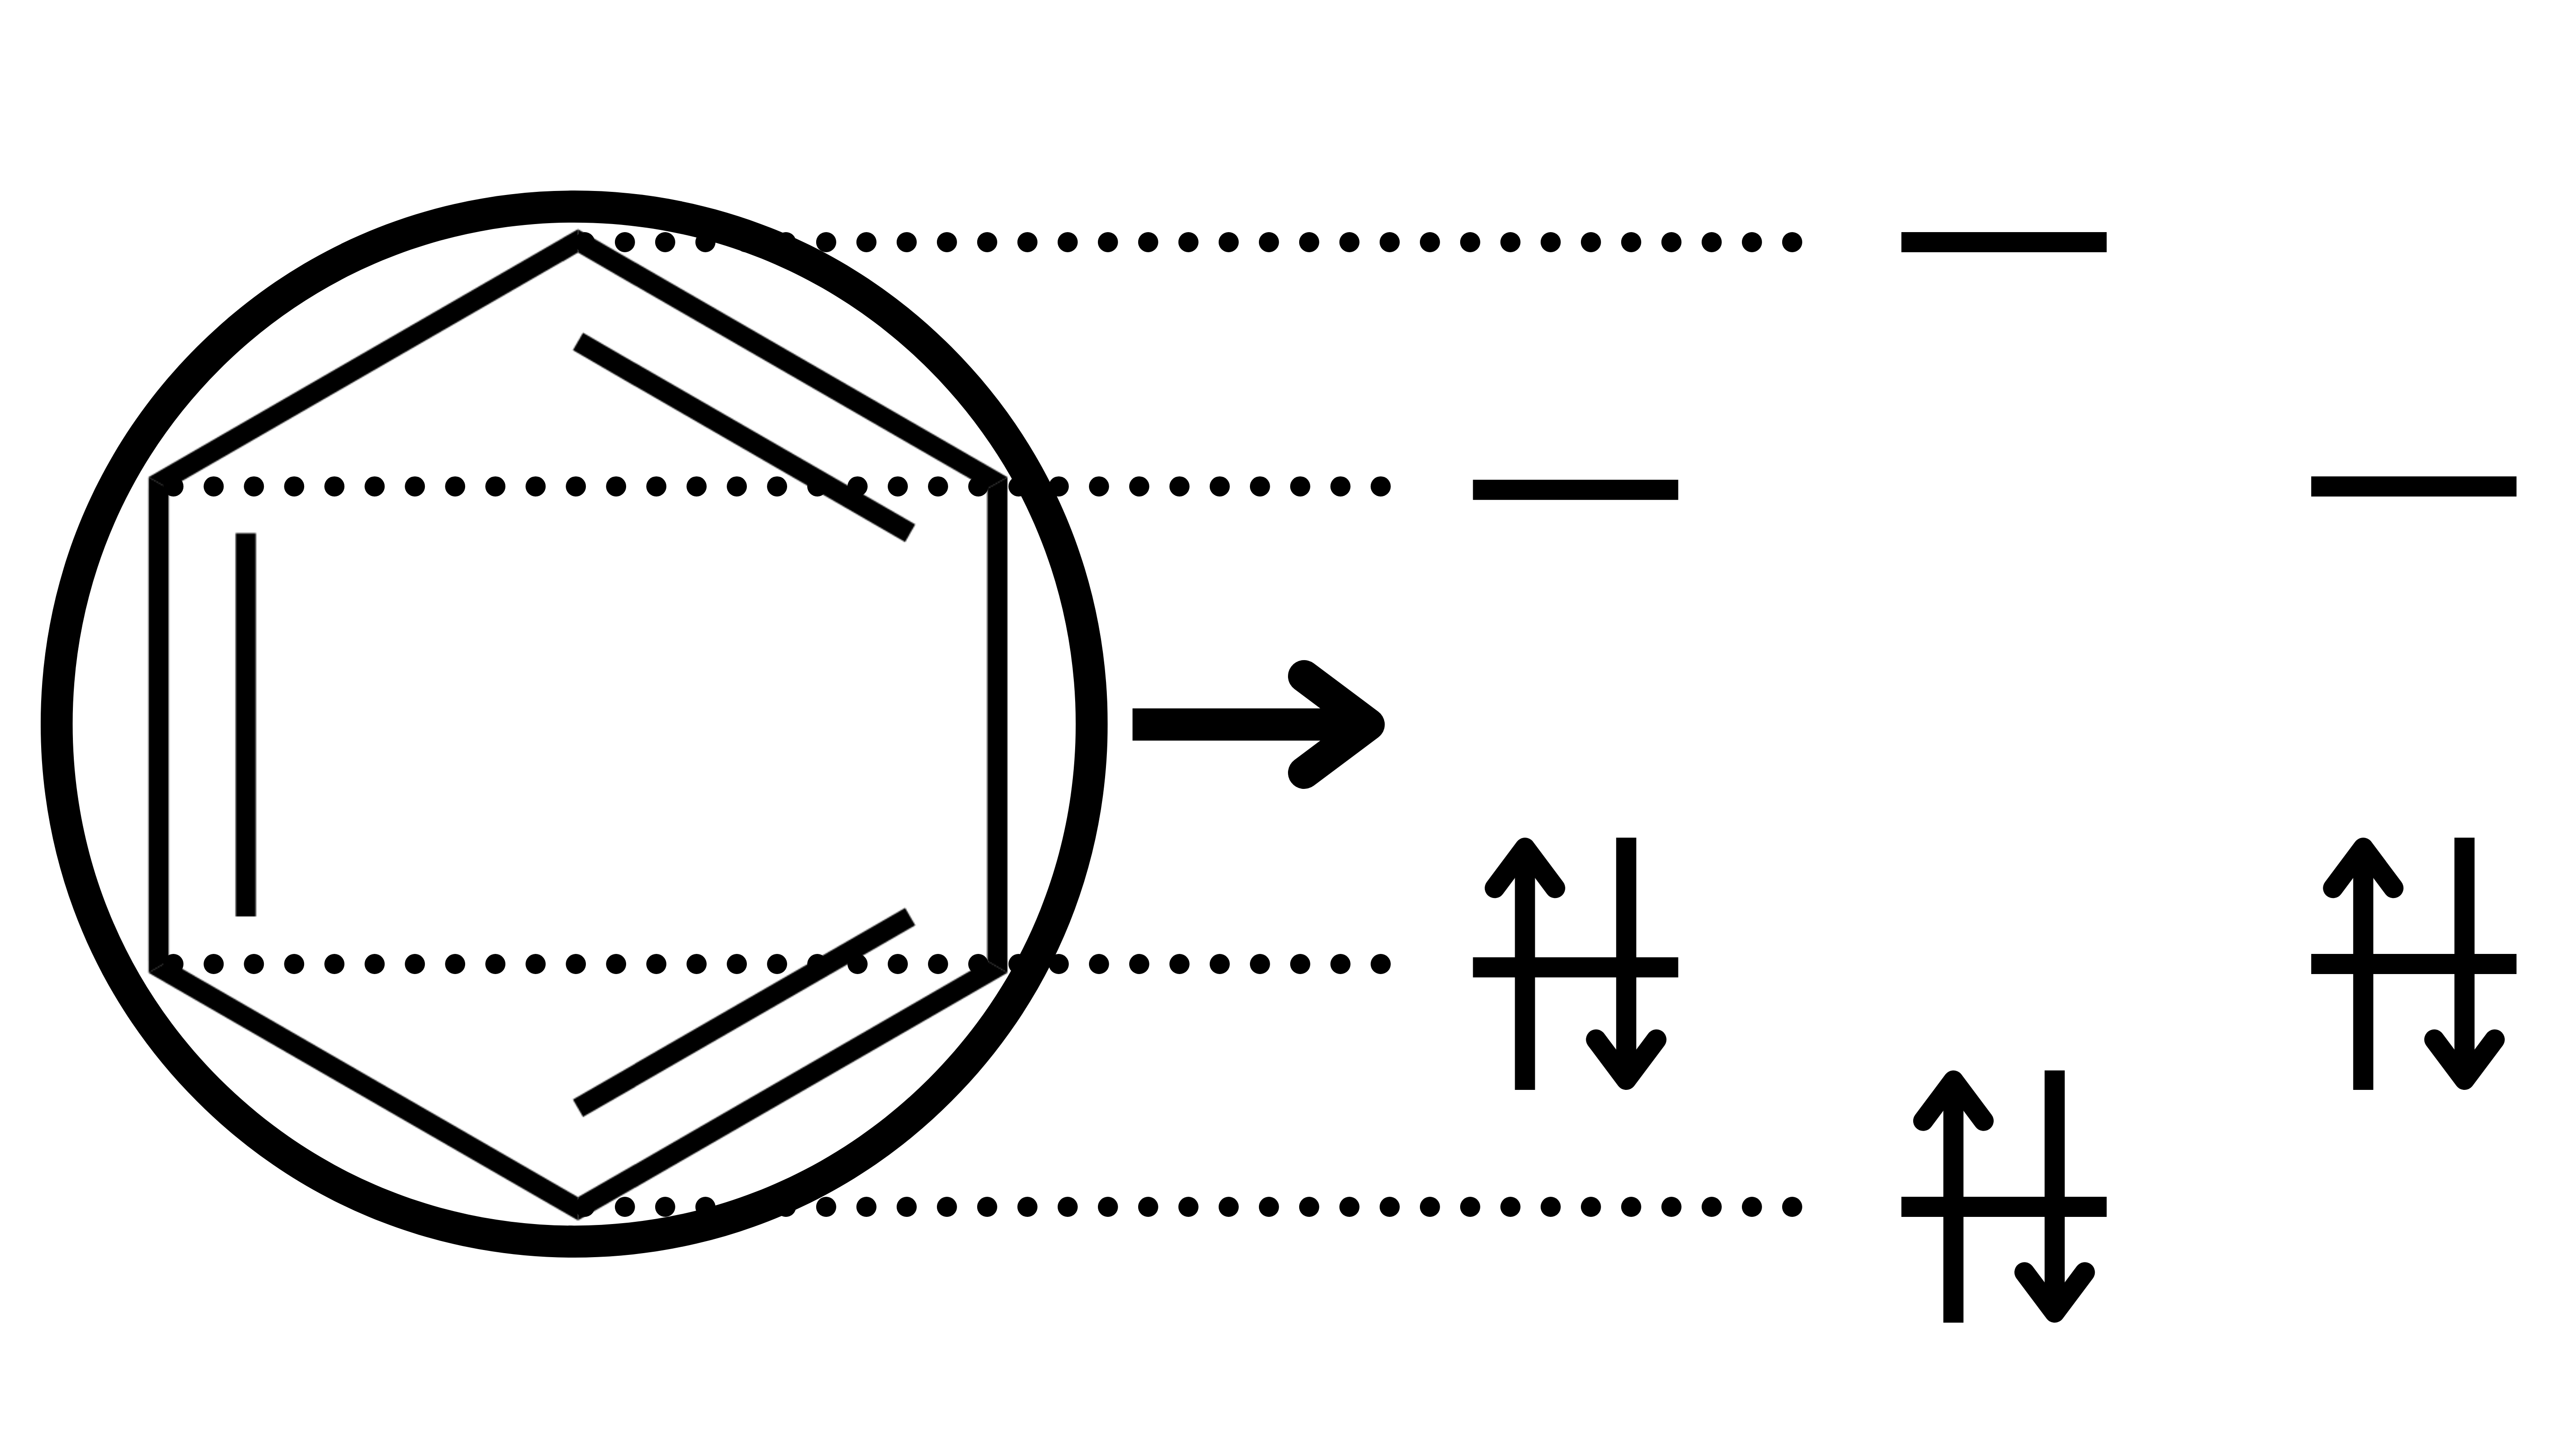
\includegraphics[width=0.60\textwidth]{images/figM.png}
	\end{center}
	\fonte{Autor(a).}
\end{figure}

Os valores de $H_{rs}$ são computados 

%%% TODO : FROST DIAGRAM

Posteriormente, essa teoria foi estendida para tratar moléculas com heteroátomos (aqueles diferentes do carbono e hidrogênio)\autocite{Liwschitz1963}. Uma mudança ainda maior foi feita por Roald Hoffmann \autocite{Hoffmann1963}, que desenvolveu o método \gls{EHMO}, o qual inclui todos os elétrons da valência (inclusive elétrons $\sigma$) no cálculo das energias dos orbitais moleculares. Esse método é classificado como semiempírico, ou seja, utiliza dados experimentais para facilitar o processo de cálculo das integrais que acessam a interação elétron-elétron para contabilizar os efeitos de correlação eletrônica na estrutura química.

Como o objetivo do trabalho é desenvolver uma ferramenta rápida e eficiente para ser utilizada dentro no navegador de internet, tal método foi escolhido pelo seu baixo custo computacional de operação, devido às aproximações das matrizes Hamiltonianas pelo teorema de Koopman, cujas consequências fazem os valores de $H_{ii}$ serem substituídos pelas energias de ionização (leia o \autoref{ap:EHMO} para mais detalhes).

A metodologia de Hueckel estendido considera todos os elétrons da valência no cálculo, e baseia-se no princípio de que os orbitais moleculares são combinações de orbitais atômicos. Desse modo, os conjuntos de base mínimos utilizados para esse procedimento são os mesmos parâmetros empregados no \gls{YAeHMOP}\autocite{Avery2017}. 

\begin{figure}[htb]
    \vspace{2\baselineskip}
\begin{equation}
    \label{eq:LCAO}
    \tikzmarknode{lcao}{\highlight{red}{LCAO}} \Longrightarrow \psi_j = \sum_{r=1}^{N} c_{jr} \tikzmarknode{aos}{\highlight{blue}{$\phi_r$}}
\end{equation}
\begin{tikzpicture}[overlay,remember picture,>=stealth,nodes={align=left,inner ysep=1pt},<-]
    \path (lcao.north) ++ (-0.70,1.5em) node[anchor=south east,color=red!67] (scalep){\textit{combinação linear}};
    \draw [color=red!87](lcao.north) |- ([xshift=-0.70em,color=red]scalep.south west);
    
    \path (aos.south) ++ (-1,-1.5em) node[anchor=north east,color=blue!67] (scalep){\textit{orbitais atômicos (conjuntos de bases)}};
    \draw [color=blue!87](aos.south) |- ([xshift=-1.65em,color=blue]scalep.north west);
\end{tikzpicture}
\vspace{2\baselineskip}
\end{figure}

A energia do j-ésimo orbital é dada pela equação monoeletrônica de Schroedinger usando um Hamiltoniano ($h_{eff}$), que expressa a interação de um elétron com o restante da molécula.

\begin{equation}
    h_{eff} \psi_j = \epsilon_j \psi_j
\end{equation}

\begin{equation}
    \epsilon_j = \frac{ \displaystyle \int \psi_j  \times h_{eff} \times \psi_j d\tau}{\displaystyle \int \psi_j \times \psi_j d\tau}
\end{equation}

\begin{equation}
    \epsilon_j = \frac{ \displaystyle \bigg{\langle} \sum_{r=1}^{N} c_{jr} \psi_r \bigg{|} h_{eff} \bigg{|} \sum_{s=1}^{N} c_{js} \psi_s \bigg{\rangle}}{\displaystyle \bigg{\langle} \sum_{r=1}^{N} c_{jr} \psi_r \bigg{|} \sum_{s=1}^{N} c_{js} \psi_s \bigg{\rangle}}
\end{equation}

Dessa expressão decorrem as integrais que precisam ser calculadas no procedimento do método:

\begin{itemize}
    \item $\displaystyle S_{rs} = \langle \psi_r | \psi_j \rangle$ é a integral de sobreposição. Como estamos trabalhando com orbitais normalizados, $S_{rr} = 1$;
    
    \item $\displaystyle H_{rr} = \langle \psi_r | h_{eff} | \psi_r \rangle$ é a integral de Coulomb, aproximada pelo oposto do potencial de ionização (como é descrito no \autoref{ap:EHMO});
    
    \item $\displaystyle H_{rs} = \langle \psi_r | h_{eff} | \psi_s \rangle$ é a integral de ressonância. Essa integral nos dá a energia de um elétron na região do espaço onde as funções $\phi_r$ e, $\phi_s$ sobrepõem-se. 
\end{itemize}

%\section{Otimização de geometria}

%Predizer o arranjo mais estável dos átomos em uma molécula é uma das mais importantes tarefas na %química quântica computacional. Essencialmente, este é um problema de otimização onde a energia total %da molécula é minimizada com relação às posições dos núcleos atômicos. A geometria molecular obtida %desse cálculo é, dessa forma, um ponto de partida para inúmeras simulações de propriedades %moleculares. Se a geometria não é acurada, então quaisquer cálculos que derivam dele também podem ser %espúrios.

%Uma vez que os núcleos são muito mais pesados do que os elétrons, nós podemos tratá-los como %partículas pontuais associadas às suas respectivas posições. A partir disso, é possível afirmar que a %energia da molécula $E(x)$ depende das coordenadas nucleares $x$, as quais definem a energia de %superfície potencial. Resolver, portanto, o problema estacionário $\nabla_x E(x)$, corresponde à %otimização das coordenadas nucleares, e a partir delas é possível determinar a energia de equilíbrio %da molécula.

%No trabalho em questão, foi utilizado um método genérico (variacional) para encontrar a estrutura %situada na região de mínima energia. A ideia central desse algoritmo é considerar explicitamente o %Hamiltoniano $H(x)$ como uma observável parametrizada, que depende das coordenadas nucleares $x$. O %objetivo desse procedimento é encontrar o mínimo global da função de custo global $g(\theta, x) = < %\Psi(\theta) | H(x) | \Psi(\theta) >$.



\section{Teoria de grafos}

Ao acessar a interface gráfica, será possível ao usuário subir um arquivo de extensão .xyz, contendo as informações em coordenadas cartesianas da estrutura a ser analisada (\autoref{workflow}). O sistema de interesse será processado computacionalmente e transformado em um grafo $G$, que corresponde a uma coleção de vértices (pontos) chamados genericamente de $V$ e arestas (linhas) denotadas por $E$. Formalmente um grafo simples $G$ é definido como um par ordenado $(V(G), E(G))$, o qual consiste de um conjunto $V(G)$ de vértices $V$ não vazio e um conjunto de arestas $E(G) = E$ contendo pares não ordenados de elementos distintos de V, uma vez que cada elemento de $E(G)$ é uma linha que conecta dois pontos de $V(G)$. Para maiores detalhes sobre a teoria de grafos, acesse o \autoref{ap:graph}.

\begin{figure}[htb]
	\caption{\label{fig:M2} Exemplo ilustrativo de um grafo cíclico não direcionado. Os pontos em azul representam os seis vértices que se conectam através das linhas pretas correspondentes às arestas. O equivalente à esquerda é um anel benzênico de Kekulé, com seis átomos de carbono ocupando os nodos de um ciclo hexagonal.}
	\begin{center}
		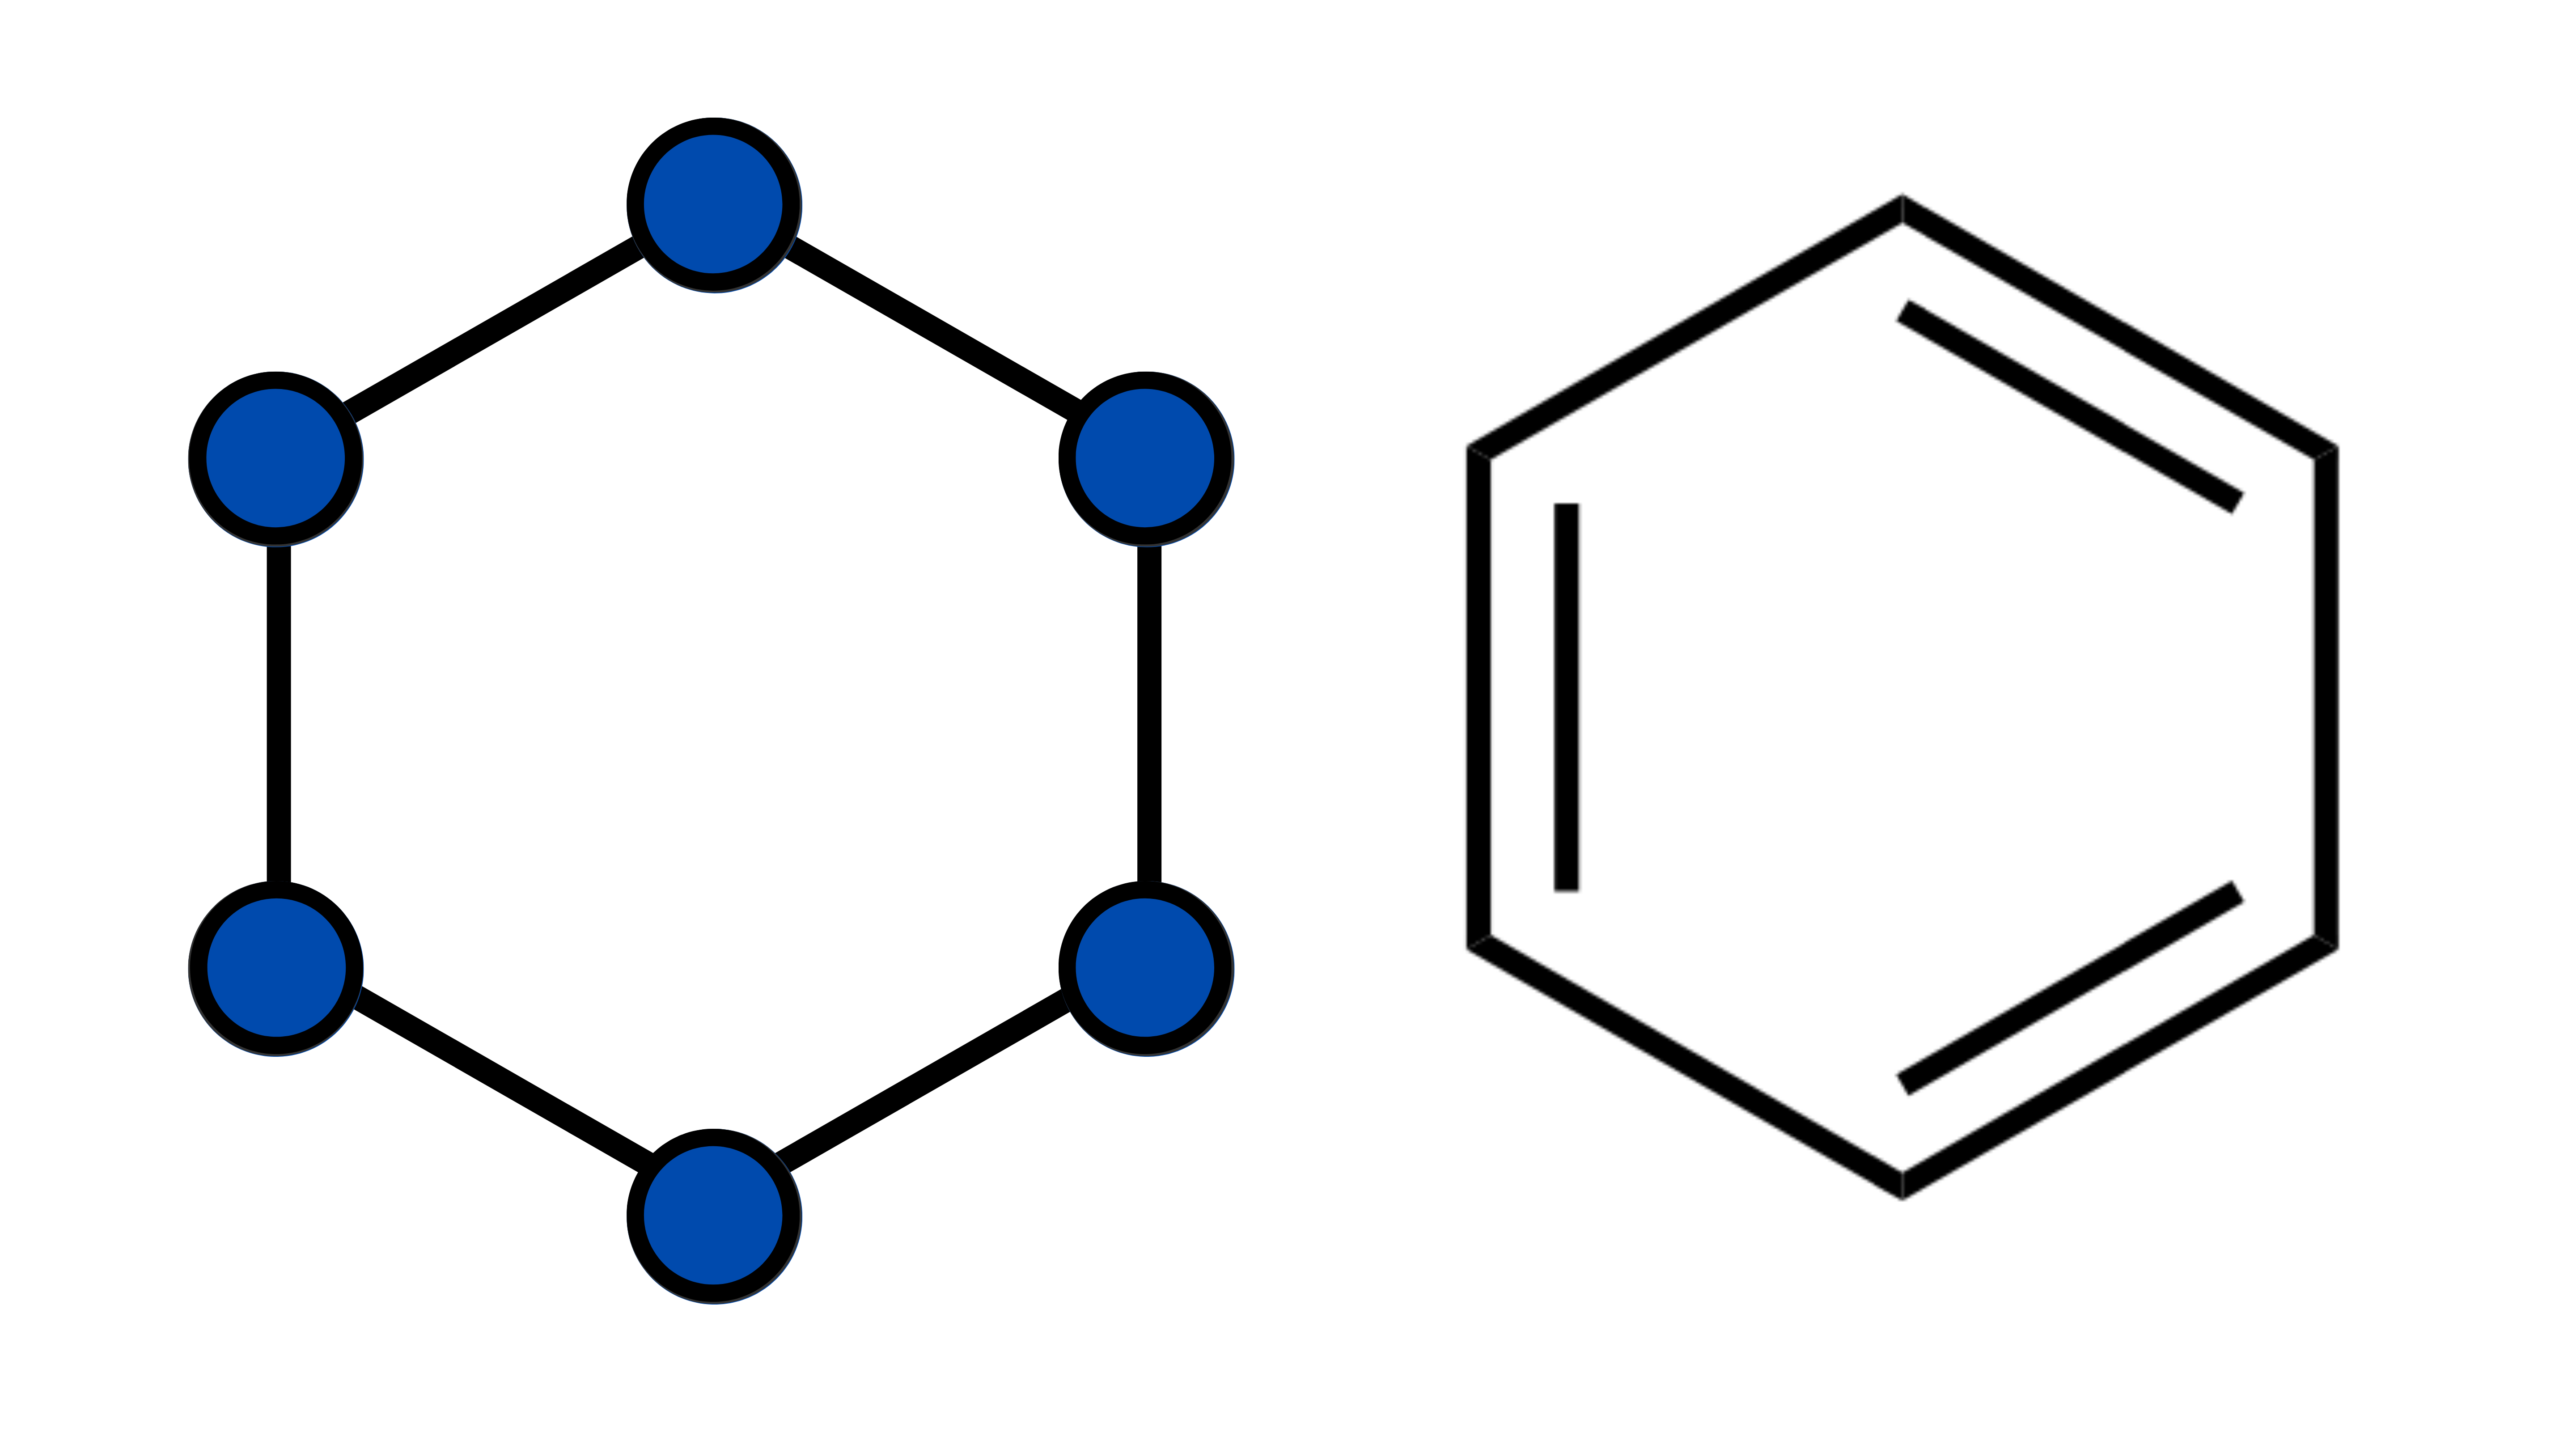
\includegraphics[width=0.65\textwidth]{images/grafo(2).png}
	\end{center}
	\fonte{Autor(a).}
\end{figure}

Desse modo, transpõe-se a representação apresentada na \autoref{fig:graph} para as estruturas químicas de interesse, uma vez que os átomos podem ser considerados os análogos químicos dos vértices, e as ligações, das arestas. Enumerando-se sequencialmente os nodos do grafo derivado do benzeno como na \autoref{fig:graphEnumerated}, é possível então verificar computacionalmente onde esses pontos estão localizados.

O DFS\autocite{Knuth1997-jf, Goodrich2001-pd} (busca em profundidade) é um algoritmo recursivo que perpassa todos os vértices de um grafo ou de uma árvore de dados através do conceito de \textit{backtracing} (retorno). Ou seja, ele começa em um nodo raiz definido arbitrariamente e a partir dele explora suas adjacências através da expansão da árvore de busca, aprofundando-se até que o alvo da busca seja encontrado ou até que ele se depare com um nó que não possui adjacências (nodo folha). Então a busca retrocede (\textit{backtrack}) e começa no próximo nó. Numa implementação não-recursiva, todos os nós expandidos recentemente são adicionados a uma pilha, para realizar a exploração (Algoritmo \ref{alg:1}, \autoref{fig:DFS}).

\begin{figure}[htb]
\caption{\label{fig:graphEnumerated}Representação do grafo mostrado na \autoref{fig:M2} com nodos enumerados sequencialmente de 1-6.}
	\begin{center}
		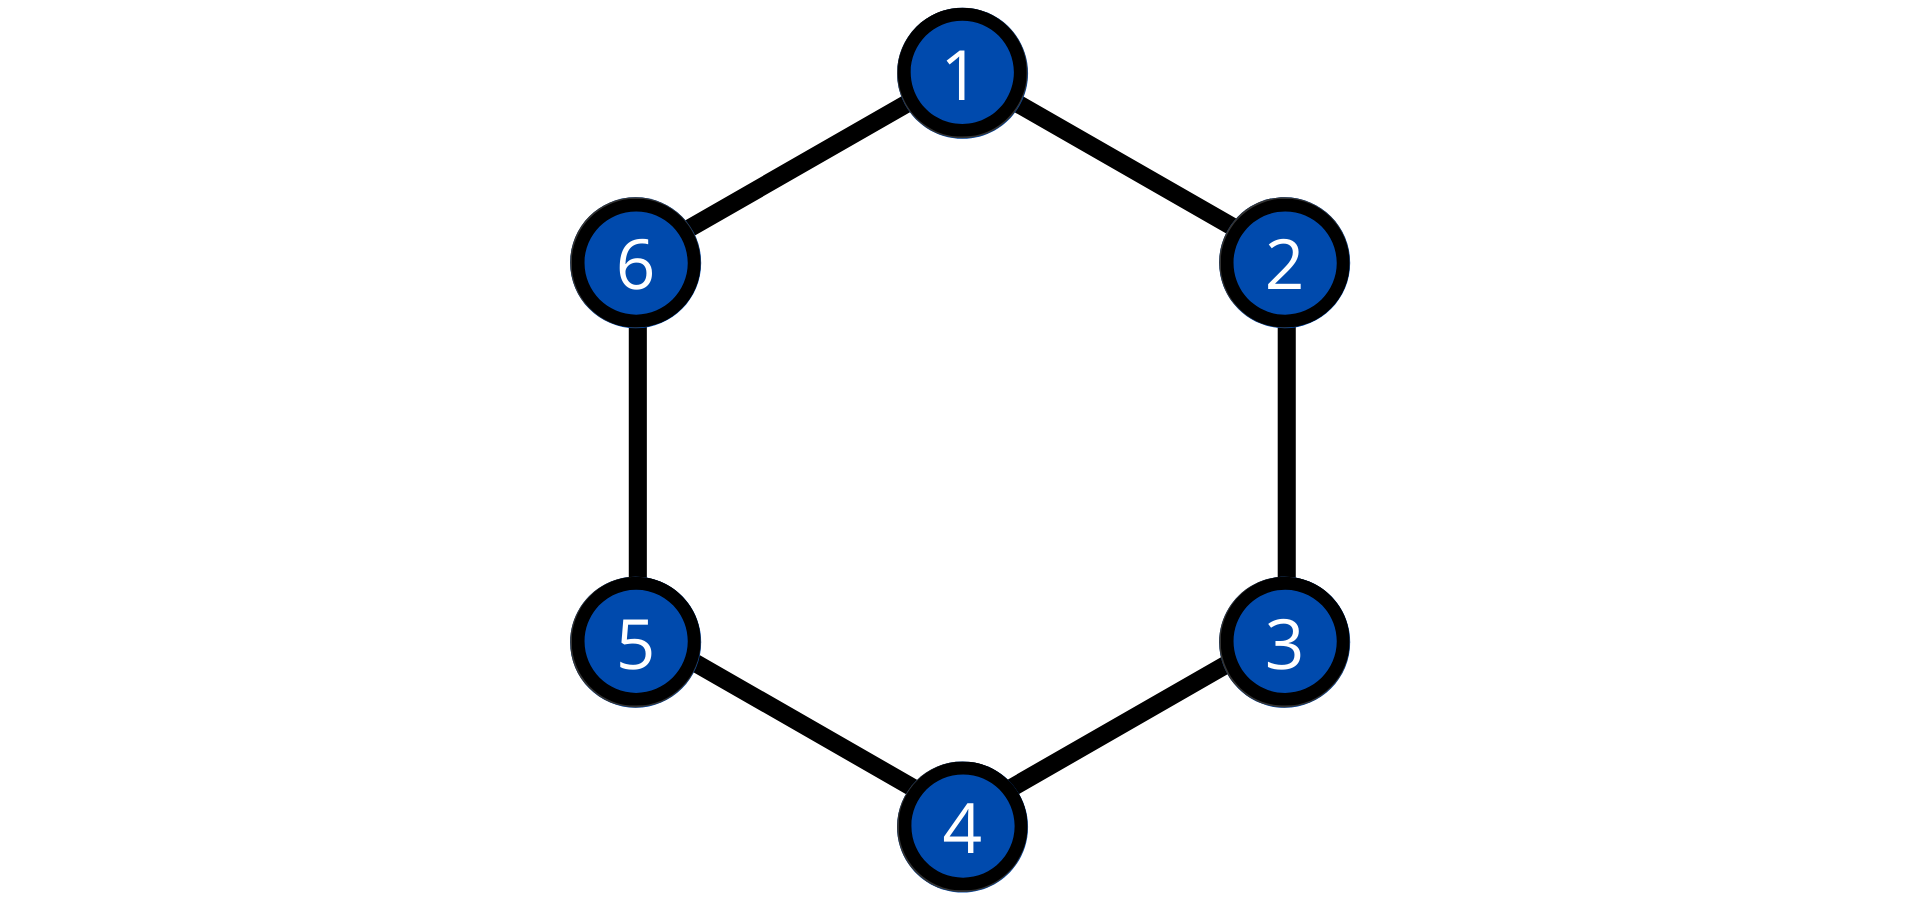
\includegraphics[width=0.65\textwidth]{images/graphEnumerated.png}
	\end{center}
	\fonte{Autor(a)}
\end{figure}

\begin{figure}[htb]
\caption{\label{fig:DFS} Representação esquemática do algoritmo DFS (Algoritmo \ref{alg:1}). Todos os nodos adjacentes são visitados até que sejam marcados como visitados (cinza). O ciclo é encontrado quando o último nodo é igual ao nodo raiz.}
	\begin{center}
		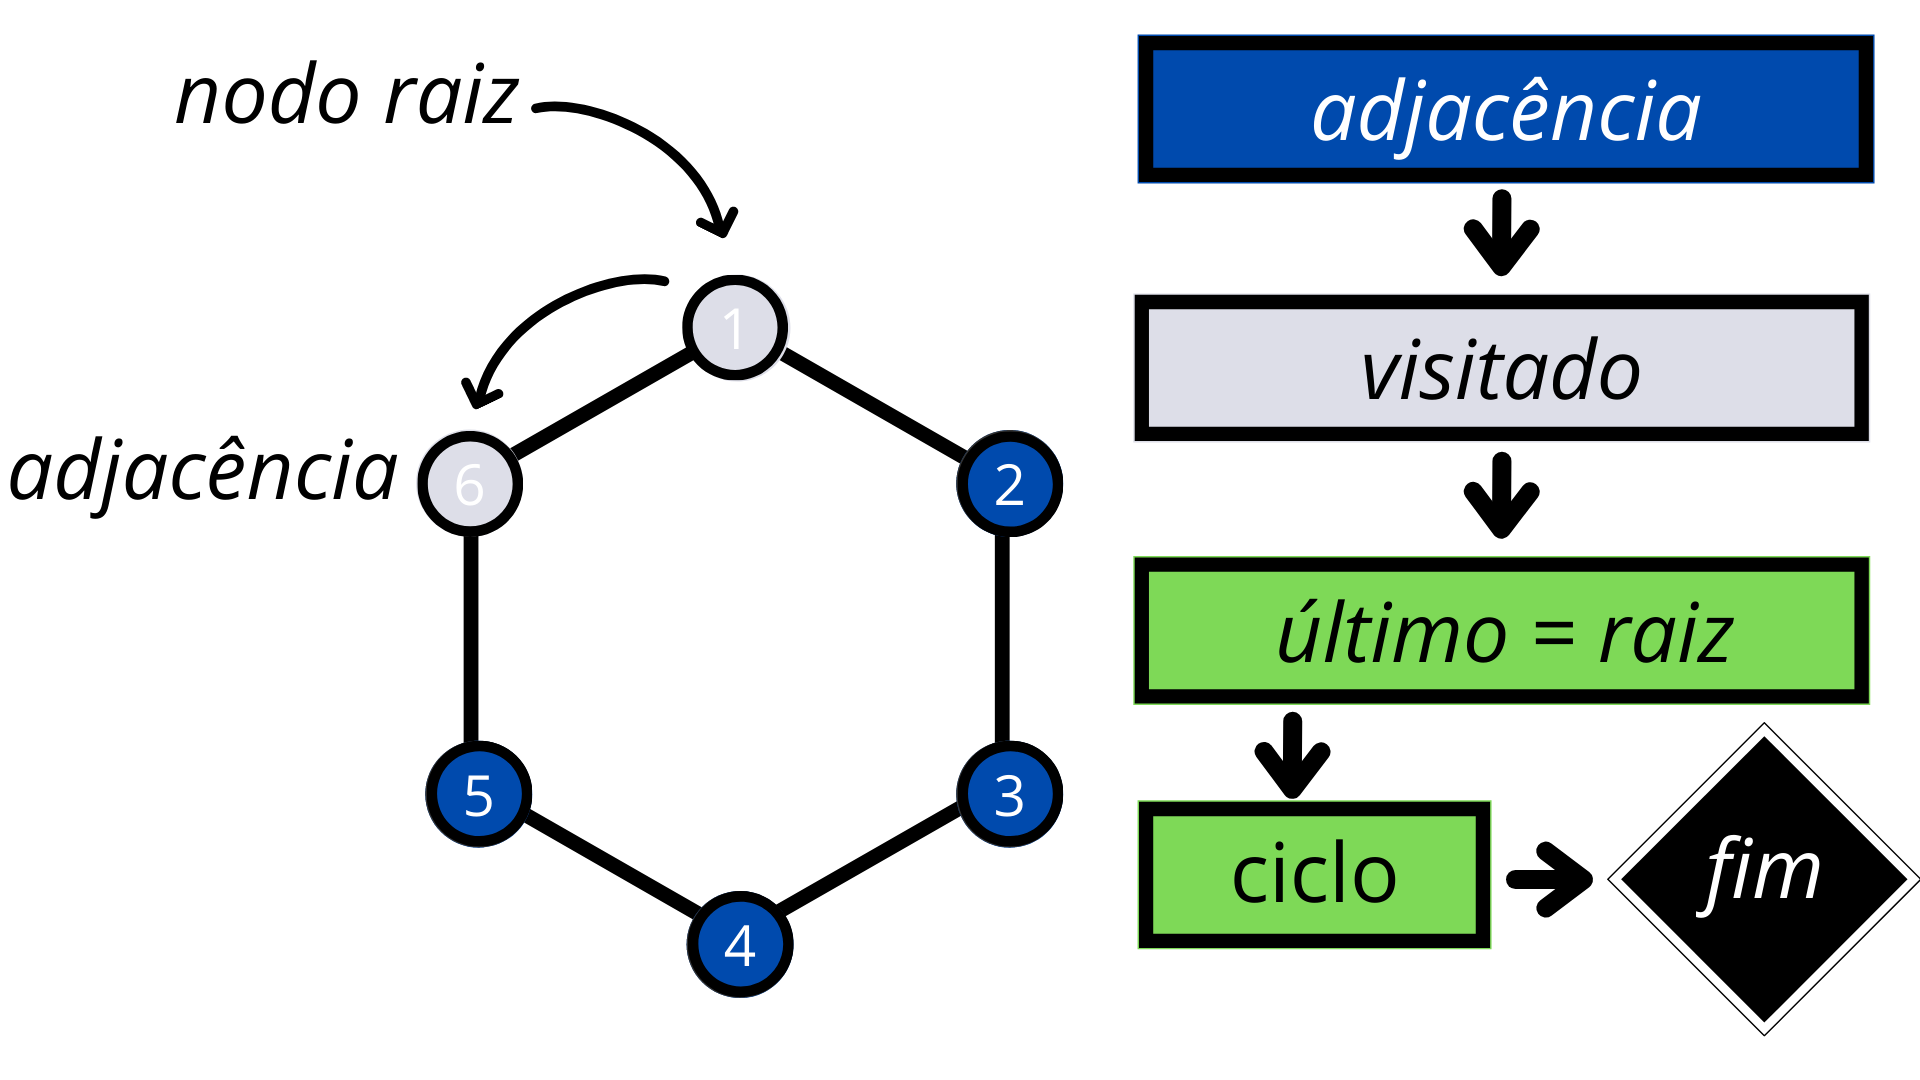
\includegraphics[width=0.75\textwidth]{images/DFS.png}
	\end{center}
	\fonte{Autor(a)}
\end{figure}

\section{Critérios quantitativos da aromaticidade}


\section{Tratamento de resíduos}

Como o trabalho em questão é teórico, foram utilizadas ferramentas computacionais dentro do Grupo de Estrutura Eletrônica Molecular (GEEM) da Universidade Federal de Santa Catarina (UFSC) para o desenvolvimento do mesmo. Desse modo, em caso de geração de lixo eletrônico, o descarte foi feito de forma apropriada junto às estações de coleta seletiva específicas, conhecidas como Ecopontos.